\documentclass[12pt]{article}

%% preamble: Keep it clean; only include those you need
\usepackage{amsmath}
\usepackage[margin = 1in]{geometry}
\usepackage{graphicx}
\usepackage{booktabs}
\usepackage{natbib}

% for space filling
\usepackage{lipsum}
% highlighting hyper links
\usepackage[colorlinks=true, citecolor=blue]{hyperref}


%% meta data

\title{STAT 3494W HW2 Stats Paper}
\author{Chris Truedson\\
  Department of Statistics\\
  University of Connecticut
}

\begin{document}
\maketitle

\begin{abstract}
\lipsum[1]
\end{abstract}


\section{Introduction}
\label{sec:intro}

Use this section to answer three questions:
Why is the topic important/interesting?
What has been done on this topic in the literature?
What is your contribution?

\lipsum[2]

To cite a reference, here are examples.
\citet{zou2006adaptive} did something ... \lipsum[1]

A lot of work has been done \citep[e.g.,][]{zou2006sparse}.
\lipsum[2]
Some parametric bootstrap sample size approach was proposed by
\citet{zou2006adaptive}. 


% roadmap
The rest of the paper is organized as follows.
The data will be presented in Section~\ref{sec:data}.
The methods are described in Section~\ref{sec:meth}.
The results are reported in Section~\ref{sec:resu}.
A discussion concludes in Section~\ref{sec:disc}.


\section{Data}
\label{sec:data}

Use this section to describe the data that helps to answer your research
questions. Recall the ideal gas law
\begin{equation}
  \label{idealgas}
  PV = nRT,
\end{equation}
which states that the $PV$ of a thing equals the product
of mass ($n$) with ($RT$).
\lipsum{1}

\section{Methods}
\label{sec:meth}

Use this section to present the methodologies that will generate results by
analyzing the data. Suppose that the radius of a circle is $r$. Then its diameter is
\begin{equation}
  \label{eq:area}
  D = 2r.
\end{equation}

Equation~\eqref{eq:area} is interesting. \lipsum[1-4]

Sometimes I don't want an equation to be numbered such as this one:
\[
  Average = \frac{\sum_{n=1}^{k}{X_{n}}}{k},
\]
which is the density of a standard normal variable.



\section{Results}
\label{sec:resu}

Table~\ref{tab:pg} Looks at Plant Growth.
\lipsum[3]

\begin{table}[tbp]
  \caption{This is my first table.}
  \label{tab:pg}
\centering
\begin{tabular}{rrl}
  \toprule
 & weight & group \\ 
  \midrule
1 & 4.17 & ctrl \\ 
  2 & 5.58 & ctrl \\ 
  3 & 5.18 & ctrl \\ 
  4 & 6.11 & ctrl \\ 
  5 & 4.50 & ctrl \\ 
  6 & 4.61 & ctrl \\ 
  7 & 5.17 & ctrl \\ 
  8 & 4.53 & ctrl \\ 
  9 & 5.33 & ctrl \\ 
  10 & 5.14 & ctrl \\ 
  11 & 4.81 & trt1 \\ 
  12 & 4.17 & trt1 \\ 
  13 & 4.41 & trt1 \\ 
  14 & 3.59 & trt1 \\ 
  15 & 5.87 & trt1 \\ 
  16 & 3.83 & trt1 \\ 
  17 & 6.03 & trt1 \\ 
  18 & 4.89 & trt1 \\ 
  19 & 4.32 & trt1 \\ 
  20 & 4.69 & trt1 \\ 
  21 & 6.31 & trt2 \\ 
  22 & 5.12 & trt2 \\ 
  23 & 5.54 & trt2 \\ 
  24 & 5.50 & trt2 \\ 
  25 & 5.37 & trt2 \\ 
  26 & 5.29 & trt2 \\ 
  27 & 4.92 & trt2 \\ 
  28 & 6.15 & trt2 \\ 
  29 & 5.80 & trt2 \\ 
  30 & 5.26 & trt2 \\ 
   \bottomrule
\end{tabular}
\end{table}

Figure~\ref{fig:iris} shows petal width v sepal width.


\begin{figure}[tbp]
  \centering
  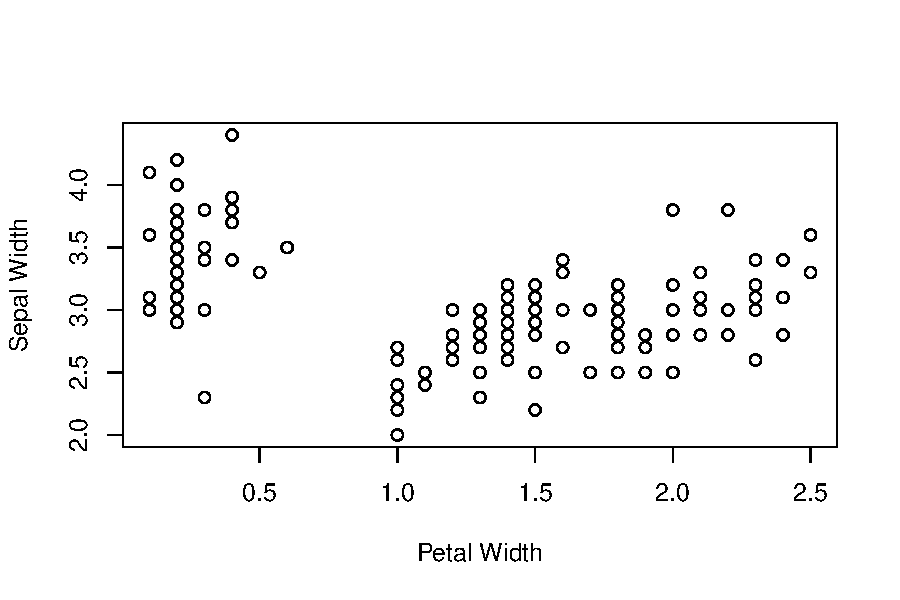
\includegraphics[width=\textwidth]{iris.pdf}
  \caption{This is my first figure for iris.}
  \label{fig:iris}
\end{figure}

\section{Discussion}
\label{sec:disc}

What are the main contributions again?

What are the limitations of this study?

What are worth pursuing further in the future?

\lipsum[1]
Watch for prevalence of diabetes \citep{yuan2006model}.

\bibliography{refs}
\bibliographystyle{mcap}

\end{document}